\section*{Background}
\subsection*{The Problem}
The interest in studying rodent whiskers has recently seen a significant increase, particularly in the field of neurophysiology. As a result, there is a need for automatic tracking of whisker movements. Currently available commercial solutions either are extremely expensive, restrict the experiment setup, or fail when whiskers cross or overlap. A cheap, reliable solution to the tracking problem is needed.

\begin{center}
  \begin{tabular}{rl}
    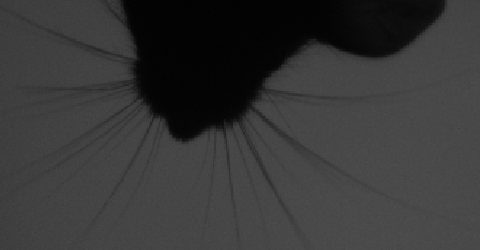
\includegraphics[width=0.15\textwidth]{rat-vanilla.png}
    & 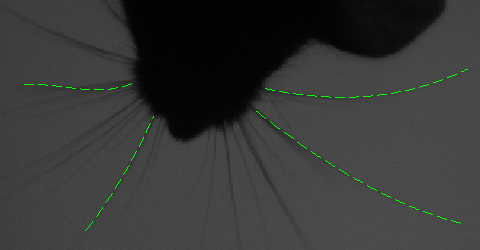
\includegraphics[width=0.15\textwidth]{rat-splines.png}
    \label{fig:rat}
  \end{tabular}
  
  Figure 1:\\
  Left: Example image of a rat and its whiskers.\\
  Right: Least squares fitted third degree polynomials.
\end{center}

\subsection*{A Probabilistic Approach}
We propose solving the problem by a probabilistic approach. We use a technique known as the \emph{Particle Filter} to propagate a whisker model between frames of high speed video. In each frame, the next state of the model is predicted by searching a pre-trained database, and filtering the results through the Particle Filter. The main difference between this and existing solutions is that it maintains a model of the whiskers. This makes it easier to keep track of them even when they cross or overlap.
